\documentclass[a4paper,11pt]{article}
\usepackage[utf8]{inputenc}
\usepackage[T1]{fontenc}
\usepackage{amsmath,amssymb}
\usepackage{geometry}
\usepackage{tikz}
\usetikzlibrary{arrows.meta}
\usepackage{enumitem}
\usepackage{fancyhdr}
\usepackage{tcolorbox}
\usepackage{pgfplots}
\pgfplotsset{compat=1.18}
\usepackage{xcolor}

\geometry{margin=2cm}
\setlength{\headheight}{14pt}

\pagestyle{fancy}
\fancyhf{}
\lhead{BTS CIEL -- Mathématiques}
\rhead{\textbf{CORRIGÉ} -- Séries de Fourier}
\cfoot{\thepage}

%% ---- Couleurs maison ----
\definecolor{vertcorr}{RGB}{0,110,60}
\definecolor{vertclair}{RGB}{220,245,230}
\definecolor{bleucorr}{RGB}{0,70,140}
\definecolor{bleuclair}{RGB}{215,230,250}
\definecolor{orangecorr}{RGB}{180,70,10}
\definecolor{orangeclair}{RGB}{255,235,210}

\tcbset{
  exobox/.style={colback=orange!5!white, colframe=orange!60!black,
                 fonttitle=\bfseries, title=#1},
  corrbox/.style={colback=vertclair, colframe=vertcorr,
                  fonttitle=\bfseries\color{vertcorr},
                  title=#1},
  formulebox/.style={colback=bleuclair, colframe=bleucorr,
                     sharp corners, boxrule=0.8pt,
                     left=5pt, right=5pt, top=4pt, bottom=4pt},
  qcmbox/.style={colback=blue!4!white, colframe=blue!50!black,
                 fonttitle=\bfseries, title=#1}
}

\newcommand{\dt}{\mathrm{d}t}
\newcommand{\reponse}[1]{%
  \begin{tcolorbox}[corrbox={}]
    #1
  \end{tcolorbox}%
}
\newcommand{\pts}[1]{\hfill\textcolor{gray}{\small\textit{(#1 pts)}}}

%% case cochée QCM
\newcommand{\coche}{\tikz[baseline=-0.5ex]{%
  \draw[vertcorr, line width=1.2pt] (0,0) rectangle (0.38,0.38);
  \draw[vertcorr, line width=1.4pt] (0.05,0.18) -- (0.16,0.05) -- (0.35,0.33);}}
\newcommand{\nocoche}{\tikz[baseline=-0.5ex]{%
  \draw[gray!50] (0,0) rectangle (0.38,0.38);}}

\begin{document}

\begin{center}
  {\LARGE \textbf{CORRIGÉ -- Évaluation Séries de Fourier}} \\[0.2cm]
  {\Large Analyse harmonique de signaux périodiques} \\[0.2cm]
  \rule{0.6\textwidth}{0.4pt} \\[0.15cm]
  \textcolor{vertcorr}{\textbf{Document réservé au professeur}}
\end{center}

\vspace{0.4cm}

% ================================================================
%  EXERCICE 1 — QCM
% ================================================================
\begin{tcolorbox}[qcmbox={Exercice 1 \, -- \, QCM \hfill \normalfont\textit{(5 points)}}]
  Réponses correctes encochées.
\end{tcolorbox}

\vspace{0.2cm}

\begin{enumerate}[label=\textbf{Q\arabic*.}, leftmargin=*, itemsep=0.4cm]

  \item $T = 5\,\mathrm{ms} = 5\times10^{-3}\,\mathrm{s}$\pts{1}

  \reponse{
    $\omega = \dfrac{2\pi}{T} = \dfrac{2\pi}{5\times10^{-3}} = 400\pi\,\mathrm{rad/s}$
    \hspace{0.5cm} \textbf{Réponse B.} \coche~$\omega = 400\pi\,\mathrm{rad/s}$
  }

  \item Propriétés d'une fonction \textbf{impaire}.\pts{1}

  \reponse{
    Si $f$ est impaire : $a_0 = 0$ et $a_n = 0$ pour tout $n \geq 1$, seuls les $b_n$ subsistent.
    \hspace{0.5cm} \textbf{Réponse B.} \coche~$a_0 = 0$ et $a_n = 0$
  }

  \item Signification de $a_0$.\pts{1}

  \reponse{
    $a_0 = \dfrac{1}{T}\displaystyle\int_0^T f(t)\,\dt$ est par définition la \textbf{valeur moyenne} du signal.
    \hspace{0.5cm} \textbf{Réponse C.} \coche~Sa valeur moyenne
  }

  \item $f(t) = 3$ sur $[0\,;\,1[$ et $f(t) = -3$ sur $[1\,;\,2[$, $T = 2$.\pts{1}

  \reponse{
    $a_0 = \dfrac{1}{2}\left[\displaystyle\int_0^1 3\,\dt + \int_1^2 (-3)\,\dt\right]
         = \dfrac{1}{2}\bigl[3\times 1 + (-3)\times 1\bigr] = \dfrac{1}{2}\times 0 = \mathbf{0}$

    \vspace{0.1cm}
    \textbf{Réponse C.} \coche~$a_0 = 0$ (signal de valeur moyenne nulle, symétrique autour de $0$)
  }

  \item Spectre en fréquences d'un signal périodique.\pts{1}

  \reponse{
    La série de Fourier est composée de termes de fréquences $f_n = n\cdot f_0$ ($n = 0,1,2,\ldots$),
    le spectre est donc constitué de \textbf{raies discrètes} aux fréquences multiples de $f_0$.
    \hspace{0.3cm} \textbf{Réponse A.} \coche~Aux fréquences $n\cdot f_0$
  }

\end{enumerate}

\vspace{0.5cm}

% ================================================================
%  EXERCICE 2 — Signal créneau asymétrique
% ================================================================
\begin{tcolorbox}[exobox={Exercice 2 \hfill \normalfont\textit{(10 points)}}]
  Signal $u$, $T = 4\,\mathrm{ms}$, $u(t)=6\,\mathrm{V}$ sur $[0\,;\,1\,\mathrm{ms}[$,
  $u(t)=0$ sur $[1\,;\,4\,\mathrm{ms}[$.
  On travaille en millisecondes ($t$ en ms), donc $\omega = \dfrac{2\pi}{4} = \dfrac{\pi}{2}\,\mathrm{rad/ms}$.
\end{tcolorbox}

\begin{enumerate}[label=\textbf{\arabic*.}, leftmargin=*, itemsep=0.4cm]

  \item Fréquence et pulsation.\pts{2}

  \reponse{
    \[
      f_0 = \frac{1}{T} = \frac{1}{4\times10^{-3}} = \mathbf{250\,\mathrm{Hz}}
    \]
    \[
      \omega = 2\pi f_0 = 2\pi \times 250 = \mathbf{500\pi \approx 1570{,}8\,\mathrm{rad/s}}
    \]
  }

  \item Calcul de $a_0$ et interprétation physique.\pts{2}

  \reponse{
    \[
      a_0 = \frac{1}{T}\int_0^{T} u(t)\,\dt
           = \frac{1}{4}\left[\int_0^{1} 6\,\dt + \int_1^{4} 0\,\dt\right]
           = \frac{1}{4}\times\bigl[6\times 1\bigr]
           = \frac{6}{4} = \mathbf{1{,}5\,\mathrm{V}}
    \]
    \textbf{Interprétation physique :} $a_0 = 1{,}5\,\mathrm{V}$ est la \textbf{composante continue}
    (valeur moyenne) du signal. En électronique, c'est la tension DC que mesurerait un voltmètre en mode DC.
    On vérifie par intuition : le signal vaut $6\,\mathrm{V}$ pendant $1/4$ de la période,
    soit $6 \times \frac{1}{4} = 1{,}5\,\mathrm{V}$.
  }

  \item Calcul de $a_n$ pour $n \geq 1$.\pts{2}

  \reponse{
    Avec $\omega = \dfrac{\pi}{2}\,\mathrm{rad/ms}$ (et $t$ en ms) :
    \begin{align*}
      a_n &= \frac{2}{T}\int_0^{T} u(t)\cos(n\omega t)\,\dt
           = \frac{2}{4}\int_0^{1} 6\cos\!\left(\frac{n\pi t}{2}\right)\dt \\[4pt]
          &= 3\left[\frac{\sin\!\left(\dfrac{n\pi t}{2}\right)}{\dfrac{n\pi}{2}}\right]_0^{1}
           = 3 \cdot \frac{2}{n\pi}\cdot\sin\!\left(\frac{n\pi}{2}\right) \\[6pt]
          &= \boxed{\frac{6}{n\pi}\sin\!\left(\frac{n\pi}{2}\right)}
    \end{align*}
    Valeurs remarquables :
    $a_1 = \dfrac{6}{\pi}\approx 1{,}91$,\quad
    $a_2 = 0$,\quad
    $a_3 = -\dfrac{2}{\pi}\approx -0{,}64$,\quad
    $a_4 = 0$, etc.
  }

  \item Calcul de $b_n$ ; valeurs de $b_1$, $b_2$, $b_3$.\pts{3}

  \reponse{
    \begin{align*}
      b_n &= \frac{2}{T}\int_0^{T} u(t)\sin(n\omega t)\,\dt
           = \frac{1}{2}\int_0^{1} 6\sin\!\left(\frac{n\pi t}{2}\right)\dt \\[4pt]
          &= 3\left[\frac{-\cos\!\left(\dfrac{n\pi t}{2}\right)}{\dfrac{n\pi}{2}}\right]_0^{1}
           = 3\cdot\frac{2}{n\pi}\left[-\cos\!\left(\frac{n\pi}{2}\right)+\cos(0)\right] \\[6pt]
          &= \boxed{\frac{6}{n\pi}\left[1-\cos\!\left(\frac{n\pi}{2}\right)\right]}
    \end{align*}

    \medskip
    \begin{itemize}[leftmargin=1.5em, itemsep=2pt]
      \item $b_1 = \dfrac{6}{\pi}\left[1-\cos\!\left(\dfrac{\pi}{2}\right)\right]
                = \dfrac{6}{\pi}\left[1-0\right] = \dfrac{6}{\pi} \approx \mathbf{1{,}91}$

      \item $b_2 = \dfrac{6}{2\pi}\left[1-\cos(\pi)\right]
                = \dfrac{3}{\pi}\left[1-(-1)\right] = \dfrac{6}{\pi} \approx \mathbf{1{,}91}$

      \item $b_3 = \dfrac{6}{3\pi}\left[1-\cos\!\left(\dfrac{3\pi}{2}\right)\right]
                = \dfrac{2}{\pi}\left[1-0\right] = \dfrac{2}{\pi} \approx \mathbf{0{,}64}$
    \end{itemize}
  }

  \item Développement tronqué à $n = 3$.\pts{1}

  \reponse{
    En substituant $a_2 = 0$, $b_2 = \dfrac{6}{\pi}$, et $\omega = 500\pi\,\mathrm{rad/s}$ :
    \[
      S(t) = 1{,}5
           + \frac{6}{\pi}\cos(\omega t)
           + \frac{6}{\pi}\sin(\omega t)
           + \frac{6}{\pi}\sin(2\omega t)
           - \frac{2}{\pi}\cos(3\omega t)
           + \frac{2}{\pi}\sin(3\omega t)
    \]
    \textit{(avec $\omega = 500\pi\,\mathrm{rad/s}$)}
  }

\end{enumerate}

\newpage

% ================================================================
%  EXERCICE 3 — Parseval et spectre
% ================================================================
\begin{tcolorbox}[exobox={Exercice 3 \hfill \normalfont\textit{(10 points)}}]
  $s(t) = 3 + 8\cos(\omega t) + 4\cos(2\omega t) + \dfrac{8}{3}\cos(3\omega t) + 2\cos(4\omega t)$,
  \quad $T = 1\,\mathrm{ms}$.
\end{tcolorbox}

\begin{enumerate}[label=\textbf{\arabic*.}, leftmargin=*, itemsep=0.4cm]

  \item Identification des coefficients.\pts{1}

  \reponse{
    Par lecture directe du développement :
    \[
      a_0 = 3, \quad a_1 = 8, \quad a_2 = 4, \quad a_3 = \frac{8}{3} \approx 2{,}67, \quad a_4 = 2
    \]
    (Tous les $b_n = 0$ : le signal est purement cosinusoïdal, donc \textbf{fonction paire}.)
  }

  \item Fréquences.\pts{1}

  \reponse{
    $T = 1\,\mathrm{ms} = 10^{-3}\,\mathrm{s}$, donc $f_0 = \dfrac{1}{T} = \mathbf{1000\,\mathrm{Hz} = 1\,\mathrm{kHz}}$.

    \medskip
    \begin{center}
    \begin{tabular}{|c|c|c|}
      \hline
      \textbf{Rang} $n$ & \textbf{Fréquence} $f_n = n\cdot f_0$ & \textbf{Terme}\\
      \hline
      0 (DC)   & $0\,\mathrm{Hz}$    & $a_0 = 3$ \\
      1 (fund.) & $1000\,\mathrm{Hz}$ & $a_1 = 8$ \\
      2         & $2000\,\mathrm{Hz}$ & $a_2 = 4$ \\
      3         & $3000\,\mathrm{Hz}$ & $a_3 = 8/3$ \\
      4         & $4000\,\mathrm{Hz}$ & $a_4 = 2$ \\
      \hline
    \end{tabular}
    \end{center}
  }

  \item Spectre unilatéral en amplitude.\pts{3}

  \reponse{
    Les raies sont à hauteur des amplitudes $|a_n|$ :

    \begin{center}
      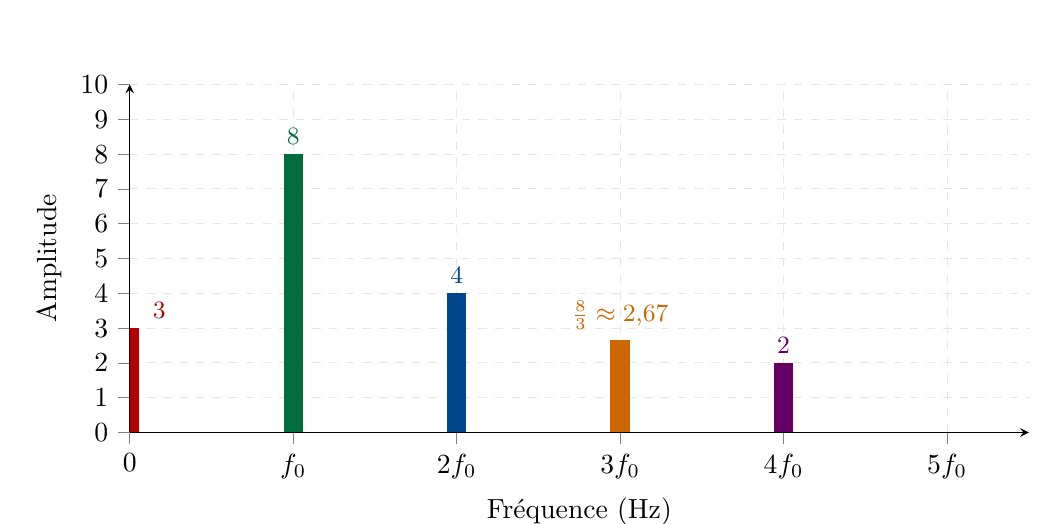
\begin{tikzpicture}
        \begin{axis}[
          axis lines=left,
          xlabel={Fréquence (Hz)},
          ylabel={Amplitude},
          xmin=0, xmax=5500,
          ymin=0, ymax=10,
          xtick={0,1000,2000,3000,4000,5000},
          xticklabels={$0$,$f_0$,$2f_0$,$3f_0$,$4f_0$,$5f_0$},
          ytick={0,1,2,3,4,5,6,7,8,9,10},
          width=13cm, height=6cm,
          grid=major,
          grid style={dashed, gray!20},
          ymajorgrids=true,
          tick align=outside,
        ]
        % Raie DC a0 = 3
        \addplot[red!70!black, line width=7pt] coordinates {(0,0)(0,3)};
        \node[above, font=\small\bfseries, red!70!black] at (axis cs:180,3) {$3$};
        % Fondamentale a1 = 8
        \addplot[vertcorr, line width=7pt] coordinates {(1000,0)(1000,8)};
        \node[above, font=\small\bfseries, vertcorr] at (axis cs:1000,8) {$8$};
        % H2 a2 = 4
        \addplot[bleucorr, line width=7pt] coordinates {(2000,0)(2000,4)};
        \node[above, font=\small\bfseries, bleucorr] at (axis cs:2000,4) {$4$};
        % H3 a3 = 8/3
        \addplot[orange!80!black, line width=7pt] coordinates {(3000,0)(3000,2.667)};
        \node[above, font=\small\bfseries, orange!80!black] at (axis cs:3000,2.667)
              {$\frac{8}{3}\approx 2{,}67$};
        % H4 a4 = 2
        \addplot[violet!80!black, line width=7pt] coordinates {(4000,0)(4000,2)};
        \node[above, font=\small\bfseries, violet!80!black] at (axis cs:4000,2) {$2$};
        \end{axis}
      \end{tikzpicture}
    \end{center}
  }

  \item Puissance de chaque composante.\pts{2}

  \reponse{
    \begin{align*}
      P_0 &= a_0^2 = 3^2 = \mathbf{9\,\mathrm{W}} \\[4pt]
      P_1 &= \frac{a_1^2}{2} = \frac{8^2}{2} = \frac{64}{2} = \mathbf{32\,\mathrm{W}} \\[4pt]
      P_2 &= \frac{a_2^2}{2} = \frac{4^2}{2} = \frac{16}{2} = \mathbf{8\,\mathrm{W}} \\[4pt]
      P_3 &= \frac{a_3^2}{2} = \frac{(8/3)^2}{2} = \frac{64/9}{2} = \frac{64}{18} = \frac{32}{9}
           \approx \mathbf{3{,}56\,\mathrm{W}} \\[4pt]
      P_4 &= \frac{a_4^2}{2} = \frac{2^2}{2} = \frac{4}{2} = \mathbf{2\,\mathrm{W}}
    \end{align*}
  }

  \item Puissance totale par Parseval.\pts{1}

  \reponse{
    \begin{align*}
      P &= P_0 + P_1 + P_2 + P_3 + P_4 \\
        &= 9 + 32 + 8 + \frac{32}{9} + 2 \\
        &= 51 + \frac{32}{9}
         = \frac{459 + 32}{9}
         = \frac{491}{9}
         \approx \mathbf{54{,}6\,\mathrm{W}}
    \end{align*}
  }

  \item Taux de distorsion harmonique (TDH).\pts{2}

  \reponse{
    \begin{align*}
      \mathrm{TDH} &= \frac{\sqrt{P_2^2 + P_3^2 + P_4^2}}{P_1}\times 100\,\%\\[6pt]
                   &= \frac{\sqrt{8^2 + \left(\dfrac{32}{9}\right)^2 + 2^2}}{32}\times 100\,\%\\[6pt]
                   &= \frac{\sqrt{64 + \dfrac{1024}{81} + 4}}{32}\times 100\,\%\\[6pt]
                   &= \frac{\sqrt{68 + 12{,}64}}{32}\times 100\,\%
                    = \frac{\sqrt{80{,}64}}{32}\times 100\,\%\\[6pt]
                   &= \frac{8{,}98}{32}\times 100\,\%
                    \approx \mathbf{28{,}1\,\%}
    \end{align*}

    \begin{tcolorbox}[colback=yellow!10!white, colframe=yellow!60!black,
                      sharp corners, boxrule=0.5pt,
                      left=5pt, right=5pt, top=3pt, bottom=3pt]
      \textbf{Commentaire :} $10\,\% \leq \mathrm{TDH} = 28{,}1\,\% \leq 30\,\%$
      \; $\Rightarrow$ \textbf{distorsion modérée}.
      Le signal présente des harmoniques significatives mais reste relativement proche d'un signal
      sinusoïdal pur. Dans un contexte électronique (alimentation, audio), ce niveau de distorsion
      serait acceptable à surveiller mais pas critique.
    \end{tcolorbox}
  }

\end{enumerate}

\end{document}
